% Yolymatics Tutorials — Hypothesis Testing Slides
% Build with: pdflatex -interaction=nonstopmode -halt-on-error hypothesis_testing_slides.tex

\documentclass[aspectratio=169,professionalfonts]{beamer}

% Core packages
\usepackage[T1]{fontenc}
\usepackage[utf8]{inputenc}
\usepackage{lmodern}
\usepackage{amsmath, amssymb}
\usepackage{graphicx}
\usepackage{booktabs}
\usepackage{microtype}
\usepackage{siunitx}
\usepackage{tikz}
\usetikzlibrary{positioning,calc,shapes,arrows.meta}
\usepackage{hyperref}

% Professional brand colors - elegant and modern
\definecolor{YolyPrimary}{HTML}{1E3A8A}   % deep professional blue
\definecolor{YolyAccent}{HTML}{F59E0B}    % warm amber
\definecolor{YolyDark}{HTML}{0F172A}      % slate dark
\definecolor{YolyLight}{HTML}{F8FAFC}     % very light gray
\definecolor{YolyMid}{HTML}{475569}       % mid slate
\definecolor{YolySecondary}{HTML}{3B82F6} % bright blue

% Beamer theme and professional styling
\mode<presentation>{
  \usetheme{Madrid}
  \usecolortheme{default}
  \setbeamertemplate{navigation symbols}{}
  
  % Main structure colors
  \setbeamercolor{structure}{fg=YolyPrimary}
  \setbeamercolor{title}{fg=white,bg=YolyPrimary}
  \setbeamercolor{frametitle}{fg=YolyDark,bg=YolyLight}
  
  % Block styling - more elegant
  \setbeamercolor{block title}{fg=white,bg=YolyPrimary}
  \setbeamercolor{block body}{fg=YolyDark,bg=YolyLight}
  \setbeamercolor{block title example}{fg=white,bg=YolyAccent}
  \setbeamercolor{block body example}{fg=YolyDark,bg=YolyLight}
  
  % Item colors
  \setbeamercolor{itemize item}{fg=YolyAccent}
  \setbeamercolor{itemize subitem}{fg=YolySecondary}
  \setbeamercolor{enumerate item}{fg=YolyAccent}
  
  % Alert color
  \setbeamercolor{alerted text}{fg=YolyAccent}
  
  % Frame title template with underline
  \setbeamertemplate{frametitle}{
    \vspace{0.3cm}
    \begin{beamercolorbox}[wd=\paperwidth,ht=1.2cm,dp=0.3cm,leftskip=0.5cm]{frametitle}
      \usebeamerfont{frametitle}\insertframetitle
      \ifx\insertframesubtitle\@empty
      \else
        \\{\small\usebeamerfont{framesubtitle}\insertframesubtitle}
      \fi
    \end{beamercolorbox}
    \vspace{-0.15cm}
    \textcolor{YolyAccent}{\rule{\paperwidth}{2pt}}
  }
  
  % Rounded blocks
  \setbeamertemplate{blocks}[rounded][shadow=false]
}

% Custom footline with brand + contact + slide count - more elegant
\setbeamertemplate{footline}{%
  \leavevmode
  \hbox{%
  \begin{beamercolorbox}[wd=.33\paperwidth,ht=2.8ex,dp=1.2ex,left]{frametitle}%
    \hspace*{1.5ex}\textbf{\textcolor{YolyPrimary}{Yolymatics Tutorials}}
  \end{beamercolorbox}%
  \begin{beamercolorbox}[wd=.34\paperwidth,ht=2.8ex,dp=1.2ex,center]{frametitle}%
    \textcolor{YolyMid}{\href{mailto:yolymatics007@gmail.com}{yolymatics007@gmail.com}}
  \end{beamercolorbox}%
  \begin{beamercolorbox}[wd=.33\paperwidth,ht=2.8ex,dp=1.2ex,right]{frametitle}%
    \textcolor{YolyMid}{\insertframenumber{} / \inserttotalframenumber}\hspace*{1.5ex}
  \end{beamercolorbox}}
  \vskip0pt}

% Professional section title page with geometric design
\AtBeginSection[]{
  \begin{frame}[plain,noframenumbering]
    \vfill
    \begin{tikzpicture}[remember picture,overlay]
      % Background accent
      \fill[YolyPrimary!10] (current page.north west) rectangle (current page.south east);
      % Geometric accent bars
      \fill[YolyPrimary] (current page.north west) rectangle ($(current page.north east)+(0,-0.5cm)$);
      \fill[YolyAccent] (current page.north west) rectangle ($(current page.north east)+(0,-0.3cm)$);
    \end{tikzpicture}
    \vspace*{4cm}
    \begin{center}
      {\usebeamerfont{title}\textcolor{YolyPrimary}{\LARGE\insertsection}}
      \vspace{0.5cm}
      
      \textcolor{YolyAccent}{\rule{0.6\linewidth}{3pt}}
    \end{center}
    \vfill
  \end{frame}}

% Title metadata
\title{Hypothesis Testing}
\subtitle{Foundations, Methods, and Examples}
\author{Yolymatics Tutorials}
\institute{\href{mailto:yolymatics007@gmail.com}{yolymatics007@gmail.com}}
\date{\today}

% Modern professional title background with geometric design
\setbeamertemplate{title page}{%
  \begin{tikzpicture}[remember picture,overlay]
    % Main blue background
    \fill[YolyPrimary] (current page.north west) rectangle ($(current page.north east)+(0,-5cm)$);
    % Accent stripe - amber
    \fill[YolyAccent] ($(current page.north west)+(0,-5cm)$) rectangle ($(current page.north east)+(0,-5.4cm)$);
    % Light background for lower section
    \fill[YolyLight] ($(current page.north west)+(0,-5.4cm)$) rectangle (current page.south east);
    
    % Geometric decorative elements
    \fill[YolySecondary,opacity=0.3] (current page.north east) circle (3cm);
    \fill[YolyAccent,opacity=0.2] ($(current page.north west)+(2cm,-2cm)$) circle (2cm);
  \end{tikzpicture}%
  
  \vspace*{2.5cm}
  \begin{flushleft}
    \hspace{0.8cm}
    {\color{white}\fontsize{32}{36}\selectfont\textbf{\inserttitle}}
    \par\vspace{0.4cm}
    \hspace{0.8cm}
    {\color{YolyLight}\Large\insertsubtitle}
  \end{flushleft}
  
  \vfill
  
  \begin{flushleft}
    \hspace{0.8cm}
    \textcolor{YolyDark}{\Large\textbf{\insertauthor}}\\[0.3ex]
    \hspace{0.8cm}
    \textcolor{YolyMid}{\large\insertinstitute}
  \end{flushleft}
  \vspace*{1cm}
}

% Convenience
\newcommand{\R}{\mathbb{R}}
\newcommand{\E}{\mathbb{E}}
\newcommand{\Var}{\mathrm{Var}}

\begin{document}

\begin{frame}[plain]
  \titlepage
\end{frame}

\begin{frame}{Today’s objectives}
  \begin{itemize}
    \item Understand the logic of hypothesis testing and key terminology
    \item Choose and run common tests (means and proportions)
    \item Interpret p-values, significance, power, and practical significance
    \item Avoid common pitfalls and clearly communicate results
  \end{itemize}
\end{frame}

\section{Big picture}

\begin{frame}{What is hypothesis testing?}
  \begin{block}{Idea}
    Use data to evaluate competing claims about a population parameter by comparing what we observed to what we'd expect if a baseline claim were true.
  \end{block}
  \vspace{0.4em}
  \begin{itemize}
    \item \textbf{Null hypothesis} $H_0$: baseline/status quo (e.g., $\mu=0$)
    \item \textbf{Alternative} $H_1$ or $H_a$: the effect/difference we care about
    \item \textbf{Test statistic}: summary of evidence (e.g., $z$, $t$)
    \item \textbf{p-value}: probability of results at least as extreme as observed if $H_0$ were true
  \end{itemize}
\end{frame}

\begin{frame}{Parameters vs. statistics}
  \begin{columns}[T,totalwidth=\textwidth]
    \begin{column}{0.50\textwidth}
      \begin{block}{Population parameter}
        \begin{itemize}
          \item Unknown quantity (e.g., mean $\mu$, proportion $p$)
          \item Fixed (does not vary across samples)
        \end{itemize}
      \end{block}
      \begin{block}{Sample statistic}
        \begin{itemize}
          \item Computed from data (e.g., $\bar x$, $\hat p$)
          \item Random (varies across samples)
        \end{itemize}
      \end{block}
    \end{column}
    \begin{column}{0.48\textwidth}
      \centering
      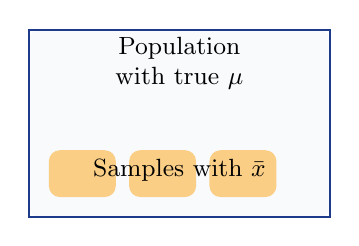
\begin{tikzpicture}[scale=0.85]
        \fill[YolyLight,rounded corners] (0,0) rectangle (4.5,2.8);
        \draw[thick, YolyPrimary] (0,0) rectangle (4.5,2.8);
        \node[align=center,font=\small] at (2.25,2.3) {Population\\with true $\mu$};
        \foreach \x in {0.3,1.5,2.7} {
          \fill[YolyAccent!50,rounded corners] (\x,0.3) rectangle +(1.0,0.7);
        }
        \node[font=\small] at (2.25,0.7) {Samples with $\bar x$};
      \end{tikzpicture}
    \end{column}
  \end{columns}
\end{frame}

\begin{frame}{Errors and decisions}
  \begin{center}
    \begin{tabular}{@{}lcc@{}}
      \toprule
      & \textbf{Fail to reject $H_0$} & \textbf{Reject $H_0$} \\
      \midrule
      $H_0$ true & Correct & \textcolor{YolyPrimary}{Type I error} ($\alpha$) \\
      $H_0$ false & \textcolor{YolyAccent!80!black}{Type II error} ($\beta$) & Correct (Power $=1-\beta$) \\
      \bottomrule
    \end{tabular}
  \end{center}
  \vspace{0.6em}
  \begin{itemize}
    \item \textbf{Significance level} $\alpha$: tolerable Type I error rate (commonly 0.05)
    \item \textbf{Power}: probability we detect a true effect (larger is better)
  \end{itemize}
\end{frame}

\begin{frame}{p-values, visually}
  \begin{columns}[T]
    \begin{column}{0.55\textwidth}
      \begin{itemize}
        \item p-value is computed assuming $H_0$ is true
        \item It is \emph{not} the probability $H_0$ is true
        \item Smaller p-value = stronger evidence against $H_0$
      \end{itemize}
    \end{column}
    \begin{column}{0.45\textwidth}
      \centering
      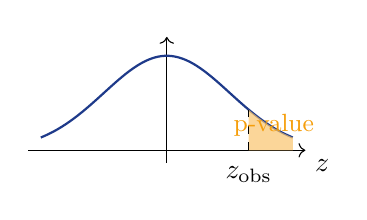
\begin{tikzpicture}[scale=0.8]
        \draw[->] (-2.2,0) -- (2.2,0) node[below right] {$z$};
        \draw[->] (0,-0.2) -- (0,1.8) node[left] {};
        % normal curve
        \draw[domain=-2:2,smooth,variable=\x,YolyPrimary,thick,samples=50] 
          plot (\x,{1.5*exp(-\x*\x/2)});
        % right tail shading
        \fill[YolyAccent!60,opacity=0.7] (1.3,0) -- 
          plot[domain=1.3:2,samples=30] (\x,{1.5*exp(-\x*\x/2)}) -- (2,0) -- cycle;
        \draw[dashed] (1.3,0) -- (1.3,{1.5*exp(-1.3*1.3/2)});
        \node[below] at (1.3,-0.1) {$z_{\text{obs}}$};
        \node[YolyAccent,font=\small] at (1.7,0.4) {p-value};
      \end{tikzpicture}
      
      \vspace{0.3em}
      {\scriptsize Shaded area = p-value (one-sided)}
    \end{column}
  \end{columns}
\end{frame}

\section{Common tests}

\begin{frame}{When to use which test?}
  \begin{block}{Decision tree for choosing tests}
    \textbf{Step 1:} What parameter are you testing?
    \begin{itemize}
      \item Mean(s) $\rightarrow$ Use z-test or t-test
      \item Proportion(s) $\rightarrow$ Use z-test for proportions
    \end{itemize}
    
    \textbf{Step 2:} How many groups?
    \begin{itemize}
      \item One group $\rightarrow$ One-sample test
      \item Two groups $\rightarrow$ Two-sample or paired test
    \end{itemize}
    
    \textbf{Step 3:} Are observations paired/matched?
    \begin{itemize}
      \item Yes (same subjects, before/after) $\rightarrow$ Paired test
      \item No (independent groups) $\rightarrow$ Independent samples test
    \end{itemize}
  \end{block}
\end{frame}

\begin{frame}{z-test vs t-test: When to use which?}
  \begin{columns}[T]
    \begin{column}{0.48\textwidth}
      \begin{block}{Use z-test when:}
        \begin{itemize}
          \item Testing \textbf{means} AND population $\sigma$ is \textbf{known}
          \item Testing \textbf{proportions} with large $n$
          \item Large sample ($n\geq 30$) AND $\sigma$ known
        \end{itemize}
      \end{block}
    \end{column}
    \begin{column}{0.48\textwidth}
      \begin{block}{Use t-test when:}
        \begin{itemize}
          \item Testing \textbf{means} AND population $\sigma$ is \textbf{unknown}
          \item Small or large sample (any $n$)
          \item Use sample SD ($s$) to estimate $\sigma$
        \end{itemize}
      \end{block}
    \end{column}
  \end{columns}
  
  \vspace{1em}
  \begin{alertblock}{Most common situation}
    In practice, $\sigma$ is usually unknown $\rightarrow$ \textbf{Use t-test for means}
  \end{alertblock}
\end{frame}

\begin{frame}{Distribution requirements}
  \begin{block}{For means (z-test or t-test)}
    \textbf{Requirements:}
    \begin{itemize}
      \item Data approximately normal, OR
      \item Large sample ($n\geq 30$) — Central Limit Theorem applies
      \item If $n<30$ with non-normal data, consider non-parametric tests
    \end{itemize}
  \end{block}
  
  \begin{block}{For proportions (z-test)}
    \textbf{Requirements (normal approximation):}
    \begin{itemize}
      \item $np_0 \geq 10$ and $n(1-p_0) \geq 10$ (one-sample)
      \item $n_1\hat p_1 \geq 10$, $n_1(1-\hat p_1) \geq 10$, and same for group 2 (two-sample)
      \item If counts too small, use exact binomial test instead
    \end{itemize}
  \end{block}
\end{frame}

\begin{frame}{General recipe}
  \begin{enumerate}
    \item State $H_0$ and $H_a$ (one- or two-sided)
    \item Choose test and check assumptions
    \item Compute test statistic
    \item Get p-value (or critical value)
    \item Conclude in context; consider effect size and CIs
  \end{enumerate}
\end{frame}

\begin{frame}{Step-by-step: Complete hypothesis testing procedure}
  \begin{block}{The 6 essential steps}
    \textbf{Step 1: State hypotheses}
    \begin{itemize}
      \item $H_0$: null hypothesis (status quo, usually "no effect" or specific value)
      \item $H_a$: alternative hypothesis (what you're trying to show)
    \end{itemize}
    
    \textbf{Step 2: Choose significance level}
    \begin{itemize}
      \item Common: $\alpha = 0.05$ or $0.01$
      \item This is your tolerance for Type I error
    \end{itemize}
    
    \textbf{Step 3: Check assumptions}
    \begin{itemize}
      \item Independence, normality (or large $n$), appropriate counts
    \end{itemize}
  \end{block}
\end{frame}

\begin{frame}{Step-by-step procedure (continued)}
  \begin{block}{Steps 4-6}
    \textbf{Step 4: Calculate test statistic}
    \begin{itemize}
      \item Use appropriate formula (z, t, etc.)
      \item This measures how far your data is from $H_0$
    \end{itemize}
    
    \textbf{Step 5: Find p-value}
    \begin{itemize}
      \item Probability of seeing data this extreme if $H_0$ were true
      \item Use tables, technology, or formulas
    \end{itemize}
    
    \textbf{Step 6: Make decision and conclude}
    \begin{itemize}
      \item Compare p-value to $\alpha$
      \item State conclusion in context of problem
    \end{itemize}
  \end{block}
\end{frame}

\begin{frame}{Decision rules: Reject or fail to reject $H_0$?}
  \begin{block}{Using p-value (most common)}
    \begin{itemize}
      \item \textbf{If p-value $\leq \alpha$}: Reject $H_0$ 
        \begin{itemize}
          \item Evidence \textit{is} strong enough against $H_0$
          \item Result is "statistically significant"
        \end{itemize}
      \item \textbf{If p-value $> \alpha$}: Fail to reject $H_0$
        \begin{itemize}
          \item Evidence \textit{is not} strong enough against $H_0$
          \item Result is "not statistically significant"
        \end{itemize}
    \end{itemize}
  \end{block}
  
  \begin{alertblock}{Important}
    We \textbf{never} "accept" $H_0$ — we only "fail to reject" it. Absence of evidence is not evidence of absence!
  \end{alertblock}
\end{frame}

\begin{frame}{Decision rules: Using critical values (alternative)}
  \begin{block}{Critical value method}
    \textbf{Step 1:} Find critical value(s) from tables based on $\alpha$
    
    \textbf{Step 2:} Compare test statistic to critical value(s)
    \begin{itemize}
      \item \textbf{Two-sided test:} Reject $H_0$ if $|$test stat$| >$ critical value
      \item \textbf{Right-tailed:} Reject $H_0$ if test stat $>$ critical value
      \item \textbf{Left-tailed:} Reject $H_0$ if test stat $<$ -critical value
    \end{itemize}
  \end{block}
  
  \vspace{0.5em}
  \textbf{Example:} For $\alpha=0.05$, two-sided z-test
  \begin{itemize}
    \item Critical values: $\pm 1.96$
    \item Reject $H_0$ if $|z| > 1.96$
  \end{itemize}
\end{frame}

\begin{frame}{One-sample z-test (mean, $\sigma$ known)}
  Assumptions: independent sample; normal population or large $n$.
  \begin{align*}
    H_0&:\ \mu=\mu_0, & H_a&:\ \mu \neq \mu_0 \ (\text{or } >, <) \\
    z&=\frac{\bar x - \mu_0}{\sigma/\sqrt{n}} \sim N(0,1)\ \text{under } H_0
  \end{align*}
  p-value: one- or two-tailed area beyond $|z|$.
\end{frame}

\begin{frame}{One-sample t-test (mean, $\sigma$ unknown)}
  Assumptions: independent; approximately normal or large $n$.
  \begin{align*}
    t=\frac{\bar x - \mu_0}{s/\sqrt{n}} \sim t_{\,n-1}\ \text{under } H_0
  \end{align*}
  Use when population SD is unknown (the usual case).
\end{frame}

\begin{frame}{Two-sample t-test (independent groups)}
  \begin{align*}
    H_0&:\ \mu_1-\mu_2=0, & H_a&:\ \mu_1-\mu_2 \neq 0 \\
    t&=\frac{(\bar x_1-\bar x_2)}{\sqrt{s_1^2/n_1 + s_2^2/n_2}} \sim t_{\,\nu}
  \end{align*}
  with Welch–Satterthwaite df $\nu$ (robust to unequal variances).
\end{frame}

\begin{frame}{Paired t-test (matched/paired data)}
  Convert to differences $d_i=x_{i,\text{after}}-x_{i,\text{before}}$ and test mean of $d$.
  \begin{align*}
    t=\frac{\bar d - 0}{s_d/\sqrt{n}} \sim t_{\,n-1}
  \end{align*}
\end{frame}

\begin{frame}{One-proportion z-test}
  Large-sample test for a single proportion.
  \begin{align*}
    H_0&:\ p=p_0, & z&=\frac{\hat p - p_0}{\sqrt{\dfrac{p_0(1-p_0)}{n}}}
  \end{align*}
  Rule of thumb: $np_0\ge 10$ and $n(1-p_0)\ge 10$.
\end{frame}

\begin{frame}{Two-proportion z-test}
  Compare two independent proportions $p_1$ and $p_2$.
  \begin{align*}
    H_0&:\ p_1-p_2=0, & z&=\frac{\hat p_1-\hat p_2}{\sqrt{\hat p(1-\hat p)(\tfrac{1}{n_1}+\tfrac{1}{n_2})}}
  \end{align*}
  where $\hat p=\dfrac{x_1+x_2}{n_1+n_2}$ is the pooled proportion under $H_0$.
\end{frame}

\section{Design, power, and sample size}

\begin{frame}{One- vs two-sided alternatives}
  \begin{itemize}
    \item Use one-sided only when effects in the other direction are \emph{impossible or irrelevant} \textit{a priori}
    \item Two-sided is more conservative and standard in most analyses
  \end{itemize}
\end{frame}

\begin{frame}{Assumptions checklist}
  \begin{itemize}
    \item Independence (study design, random sampling/assignment)
    \item Approximate normality for means (or large $n$ via CLT)
    \item Sufficient counts for proportions
    \item No severe outliers/heteroscedasticity for t-tests
  \end{itemize}
\end{frame}

\begin{frame}{Power in plain terms}
  \begin{block}{Power}
    Probability your test detects a true effect of a given size. Improves with larger effects, larger $n$, lower variability, and higher $\alpha$.
  \end{block}
  \begin{itemize}
    \item Report effect sizes (e.g., Cohen's $d$) and confidence intervals
    \item Consider practical vs. statistical significance
  \end{itemize}
\end{frame}

\begin{frame}{Back-of-envelope sample size}
  For mean with known $\sigma$ (approximate):
  \[
    n \approx \left(\frac{z_{1-\alpha/2}\,\sigma}{\mathrm{ME}}\right)^2
  \]
  For proportion (worst-case $p=0.5$):
  \[
    n \approx \frac{z_{1-\alpha/2}^2\,0.25}{\mathrm{ME}^2}
  \]
  where ME is desired half-width of CI.
\end{frame}

\section{Practice Problems}

% ========== ONE-SAMPLE TESTS ==========

\begin{frame}{Problem 1: One-sample t-test}
  \begin{block}{Problem}
    A sample of $n=25$ students has average score $\bar x=78.4$ with $s=10.2$. Test if the population mean differs from 75 at $\alpha=0.05$.
  \end{block}
  
  \vspace{1em}
  \textbf{Workspace:}
  \vspace{4cm}
\end{frame}

\begin{frame}[plain]{Problem 1: Workspace (continued)}
  \vspace{7cm}
\end{frame}

\begin{frame}{Problem 2: One-sample z-test}
  \begin{block}{Problem}
    A factory claims their bolts have a mean diameter of 5.0 mm with known $\sigma=0.12$ mm. A random sample of 40 bolts has $\bar x=5.04$ mm. Test at $\alpha=0.01$ if the true mean differs from 5.0 mm.
  \end{block}
  
  \vspace{1em}
  \textbf{Workspace:}
  \vspace{4cm}
\end{frame}

\begin{frame}[plain]{Problem 2: Workspace (continued)}
  \vspace{7cm}
\end{frame}

\begin{frame}{Problem 3: One-sided t-test}
  \begin{block}{Problem}
    A new teaching method is tested with 18 students. Their mean score is 82.5 with $s=9.8$. The traditional method has a mean of 78. Test if the new method is better at $\alpha=0.05$.
  \end{block}
  
  \vspace{1em}
  \textbf{Workspace:}
  \vspace{4cm}
\end{frame}

\begin{frame}[plain]{Problem 3: Workspace (continued)}
  \vspace{7cm}
\end{frame}

% ========== TWO-SAMPLE TESTS ==========

\begin{frame}{Problem 4: Two-sample t-test}
  \begin{block}{Problem}
    Group 1: $n_1=30$, $\bar x_1=72$, $s_1=8$\\
    Group 2: $n_2=28$, $\bar x_2=68$, $s_2=9$\\
    Test if the means differ at $\alpha=0.05$.
  \end{block}
  
  \vspace{1em}
  \textbf{Workspace:}
  \vspace{4cm}
\end{frame}

\begin{frame}[plain]{Problem 4: Workspace (continued)}
  \vspace{7cm}
\end{frame}

\begin{frame}{Problem 5: Two-sample comparison}
  \begin{block}{Problem}
    Two brands of batteries are tested. Brand A ($n=35$): $\bar x=42.3$ hours, $s=5.2$ hours. Brand B ($n=40$): $\bar x=39.8$ hours, $s=6.1$ hours. Is there evidence Brand A lasts longer? Use $\alpha=0.05$.
  \end{block}
  
  \vspace{1em}
  \textbf{Workspace:}
  \vspace{3.5cm}
\end{frame}

\begin{frame}[plain]{Problem 5: Workspace (continued)}
  \vspace{7cm}
\end{frame}

% ========== PAIRED TESTS ==========

\begin{frame}{Problem 6: Paired t-test}
  \begin{block}{Problem}
    10 patients' blood pressure before and after treatment:\\
    Differences (After - Before): $-8, -12, -5, -9, -15, -7, -11, -6, -10, -13$\\
    Test if treatment reduces blood pressure at $\alpha=0.05$.
  \end{block}
  
  \vspace{1em}
  \textbf{Workspace:}
  \vspace{3.5cm}
\end{frame}

\begin{frame}[plain]{Problem 6: Workspace (continued)}
  \vspace{7cm}
\end{frame}

\begin{frame}{Problem 7: Paired data analysis}
  \begin{block}{Problem}
    12 students take a test before and after tutoring. The mean difference is $\bar d = 7.5$ points with $s_d=4.2$. Test if tutoring improves scores at $\alpha=0.01$.
  \end{block}
  
  \vspace{1em}
  \textbf{Workspace:}
  \vspace{4cm}
\end{frame}

\begin{frame}[plain]{Problem 7: Workspace (continued)}
  \vspace{7cm}
\end{frame}

% ========== PROPORTION TESTS ==========

\begin{frame}{Problem 8: One-proportion z-test}
  \begin{block}{Problem}
    In $n=200$ trials, $x=118$ successes ($\hat p=0.59$). Test $H_0:p=0.5$ vs $H_a:p\neq 0.5$ at $\alpha=0.05$.
  \end{block}
  
  \vspace{1em}
  \textbf{Workspace:}
  \vspace{4cm}
\end{frame}

\begin{frame}[plain]{Problem 8: Workspace (continued)}
  \vspace{7cm}
\end{frame}

\begin{frame}{Problem 9: Proportion test (one-sided)}
  \begin{block}{Problem}
    A company claims that more than 30\% of customers prefer their product. In a survey of 150 customers, 54 prefer it. Test the claim at $\alpha=0.05$.
  \end{block}
  
  \vspace{1em}
  \textbf{Workspace:}
  \vspace{4cm}
\end{frame}

\begin{frame}[plain]{Problem 9: Workspace (continued)}
  \vspace{7cm}
\end{frame}

\begin{frame}{Problem 10: Two-proportion z-test}
  \begin{block}{Problem}
    Treatment A: 45 successes out of 100 trials\\
    Treatment B: 38 successes out of 90 trials\\
    Test if the success rates differ at $\alpha=0.05$.
  \end{block}
  
  \vspace{1em}
  \textbf{Workspace:}
  \vspace{4cm}
\end{frame}

\begin{frame}[plain]{Problem 10: Workspace (continued)}
  \vspace{7cm}
\end{frame}

\begin{frame}{Problem 11: Comparing proportions}
  \begin{block}{Problem}
    Male voters: 132 out of 200 support a policy\\
    Female voters: 145 out of 220 support the policy\\
    Is there evidence of a gender difference in support? Use $\alpha=0.01$.
  \end{block}
  
  \vspace{1em}
  \textbf{Workspace:}
  \vspace{3.5cm}
\end{frame}

\begin{frame}[plain]{Problem 11: Workspace (continued)}
  \vspace{7cm}
\end{frame}

% ========== INTERPRETATION & ASSUMPTIONS ==========

\begin{frame}{Problem 12: P-value interpretation}
  \begin{block}{Problem}
    A hypothesis test yields $p=0.032$.
    \begin{enumerate}
      \item What does this p-value mean in context?
      \item What decision would you make at $\alpha=0.05$?
      \item What decision would you make at $\alpha=0.01$?
      \item Does this prove the null hypothesis is false?
    \end{enumerate}
  \end{block}
  
  \vspace{1em}
  \textbf{Workspace:}
  \vspace{2.5cm}
\end{frame}

\begin{frame}[plain]{Problem 12: Workspace (continued)}
  \vspace{7cm}
\end{frame}

\begin{frame}{Problem 13: Type I and II errors}
  \begin{block}{Problem}
    A drug company tests if a new drug reduces cholesterol.
    \begin{enumerate}
      \item State the null and alternative hypotheses
      \item Describe a Type I error in context
      \item Describe a Type II error in context
      \item Which error is more serious? Explain.
    \end{enumerate}
  \end{block}
  
  \vspace{1em}
  \textbf{Workspace:}
  \vspace{2cm}
\end{frame}

\begin{frame}[plain]{Problem 13: Workspace (continued)}
  \vspace{7cm}
\end{frame}

\begin{frame}{Problem 14: Assumptions check}
  \begin{block}{Problem}
    You want to perform a one-sample t-test on a sample of $n=12$ data points. The data shows strong right skewness and contains one extreme outlier.
    \begin{enumerate}
      \item Are the t-test assumptions met?
      \item What could you do instead?
      \item If you had $n=100$ with the same skewness, would that change your answer?
    \end{enumerate}
  \end{block}
  
  \vspace{1em}
  \textbf{Workspace:}
  \vspace{2cm}
\end{frame}

\begin{frame}[plain]{Problem 14: Workspace (continued)}
  \vspace{7cm}
\end{frame}

% ========== POWER & SAMPLE SIZE ==========

\begin{frame}{Problem 15: Sample size calculation}
  \begin{block}{Problem}
    You want to estimate a population proportion with margin of error $\pm 0.04$ at 95\% confidence. Calculate the required sample size assuming:
    \begin{enumerate}
      \item Worst-case scenario ($p=0.5$)
      \item Previous estimate suggests $p=0.3$
    \end{enumerate}
  \end{block}
  
  \vspace{1em}
  \textbf{Workspace:}
  \vspace{3cm}
\end{frame}

\begin{frame}[plain]{Problem 15: Workspace (continued)}
  \vspace{7cm}
\end{frame}

\begin{frame}{Problem 16: Power concepts}
  \begin{block}{Problem}
    \begin{enumerate}
      \item If you decrease $\alpha$ from 0.05 to 0.01, what happens to power?
      \item If you increase sample size, what happens to power?
      \item If the true effect size is larger, what happens to power?
      \item A test has power = 0.85. What does this mean?
    \end{enumerate}
  \end{block}
  
  \vspace{1em}
  \textbf{Workspace:}
  \vspace{2.5cm}
\end{frame}

\begin{frame}[plain]{Problem 16: Workspace (continued)}
  \vspace{7cm}
\end{frame}

% ========== COMPREHENSIVE PROBLEMS ==========

\begin{frame}{Problem 17: Complete analysis (means)}
  \begin{block}{Problem}
    A researcher claims a new diet reduces weight. 20 people follow the diet for 8 weeks. Weight loss (kg): Mean = 3.8, SD = 2.1.
    \begin{enumerate}
      \item State appropriate hypotheses
      \item Check assumptions
      \item Compute test statistic
      \item Find p-value and conclude at $\alpha=0.05$
      \item Calculate a 95\% confidence interval
    \end{enumerate}
  \end{block}
  
  \vspace{1em}
  \textbf{Workspace:}
  \vspace{1.5cm}
\end{frame}

\begin{frame}[plain]{Problem 17: Workspace (continued)}
  \vspace{7cm}
\end{frame}

\begin{frame}[plain]{Problem 17: Workspace (continued 2)}
  \vspace{7cm}
\end{frame}

\begin{frame}{Problem 18: Complete analysis (proportions)}
  \begin{block}{Problem}
    Before campaign: 120 out of 300 people support a policy (40\%)\\
    After campaign: 145 out of 280 people support it (51.8\%)
    \begin{enumerate}
      \item State hypotheses for testing if support increased
      \item Conduct appropriate test at $\alpha=0.05$
      \item Calculate effect size
      \item Is the result practically significant?
    \end{enumerate}
  \end{block}
  
  \vspace{1em}
  \textbf{Workspace:}
  \vspace{2cm}
\end{frame}

\begin{frame}[plain]{Problem 18: Workspace (continued)}
  \vspace{7cm}
\end{frame}

\begin{frame}[plain]{Problem 18: Workspace (continued 2)}
  \vspace{7cm}
\end{frame}

\begin{frame}{Problem 19: Critical thinking}
  \begin{block}{Problem}
    A study tests 50 different hypotheses and finds 3 significant results at $\alpha=0.05$.
    \begin{enumerate}
      \item How many would you expect by chance alone?
      \item What problem does this illustrate?
      \item What should the researchers do?
    \end{enumerate}
  \end{block}
  
  \vspace{1em}
  \textbf{Workspace:}
  \vspace{3.5cm}
\end{frame}

\begin{frame}[plain]{Problem 19: Workspace (continued)}
  \vspace{7cm}
\end{frame}

\begin{frame}{Problem 20: Design a study}
  \begin{block}{Problem}
    You want to test if a new app improves math scores. Design a study including:
    \begin{enumerate}
      \item Null and alternative hypotheses
      \item Type of test you'll use
      \item Sample size justification
      \item How you'll minimize bias
      \item What you'll report beyond just p-values
    \end{enumerate}
  \end{block}
  
  \vspace{1em}
  \textbf{Workspace:}
  \vspace{1.5cm}
\end{frame}

\begin{frame}[plain]{Problem 20: Workspace (continued)}
  \vspace{7cm}
\end{frame}

\begin{frame}[plain]{Problem 20: Workspace (continued 2)}
  \vspace{7cm}
\end{frame}

\section{Communication}

\begin{frame}{Interpreting p-values (do and don't)}
  \begin{itemize}
    \item Do: "If $H_0$ were true, we'd see results this extreme only about 1% of the time."
    \item Don't: "The probability $H_0$ is true is 1%." (that's incorrect)
    \item Report effect size and CI; avoid dichotomizing by 0.05 alone
  \end{itemize}
\end{frame}

\begin{frame}{Common pitfalls}
  \begin{itemize}
    \item P-hacking and multiple testing without correction
    \item Ignoring assumptions or study design
    \item Confusing absence of evidence with evidence of absence
    \item Over-reliance on arbitrary significance thresholds
    \item Ignoring effect sizes and practical significance
  \end{itemize}
\end{frame}

\begin{frame}[plain,noframenumbering]
  \begin{tikzpicture}[remember picture,overlay]
    \fill[YolyPrimary] (current page.north west) rectangle (current page.south east);
    \fill[YolyAccent,opacity=0.2] (current page.north east) circle (4cm);
    \fill[YolySecondary,opacity=0.15] ($(current page.south west)+(3cm,3cm)$) circle (3cm);
  \end{tikzpicture}
  \vfill
  \begin{center}
    {\color{white}\Huge\textbf{Thank you!}}\\[1cm]
    {\color{YolyLight}\LARGE\textbf{Yolymatics Tutorials}}\\[0.5cm]
    {\color{YolyLight}\Large\href{mailto:yolymatics007@gmail.com}{yolymatics007@gmail.com}}\\[1.5cm]
    {\color{YolyAccent}\Large Keep practicing and stay curious!}
  \end{center}
  \vfill
\end{frame}

\end{document}
